\documentclass{article}

\usepackage{amsmath, amssymb}
\usepackage{xcolor}
\usepackage{caption, subcaption}
\usepackage{graphicx}
\usepackage{bm}             % For bold math symbols
\usepackage{soul}
\usepackage{outlines}   % For multilevel lists using the outline environment
\usepackage{tikz}
\usetikzlibrary{arrows.meta, positioning}


\usepackage{natbib}
\bibliographystyle{plainnat}

\usepackage{hyperref}   % For the \url{} command


\newcommand{\bG}{\mathbb{G}}
\newcommand{\bF}{\mathbb{F}}
\newcommand{\bP}{\mathbb{P}}
\newcommand{\bE}{\mathbb{E}}
\newcommand{\bV}{\mathbb{V}}

\newcommand{\zdens}{\frac{e^{-z^2/2}}{\sqrt{2\pi}}}
\newcommand{\indep}{\perp \!\!\! \perp}


\title{Analytical Uncertainty Quantification for Multilevel Mediation Analysis}

\begin{document}

\maketitle
\section{Notes to Self}
\begin{outline}
    \1 In the paper, I organize variables as $Y, X, M, W$. This is based on defining counterfactuals as $Y_x$, then adding $M$, giving $Y_{x, m}$. In my code, it's always $Y, M, X, W$. I must be very careful to not mess this ordering up. The code is more arbitrary, but it's also harder to change. For now, I'm just going to try to juggle this difference manually, but I will need to carefully validate any results when passing from code to paper (this sort of issue has already been the source of one elusive error in my code).
    \1 I need to be very explicit that our analysis of expected counterfactuals is in service to mediation effects. Once we have estimates and UQ for expected counterfactuals, the extension to total, direct and indirect effects is straightforward.
\end{outline}



\section{Introduction}

Mediation analysis is a central problem in modern causal inference. Many scientific and public health questions have the form of separating the direct effect of some exposure on an outcome from the indirect effect of that exposure via a mediator. Many authors have developed methods to address this problem; gradually increasing in complexity. Early work by \citet{Bar86} laid the foundation for future developments, but did not use the machinery of counterfactual outcomes. 

There have been several approaches to the analysis of causal mediation. One group established a non-parametric identification result \citep{Ima10II}, and used this result to estimate mediation effects in various contexts \citep{Ima10I, Ima11}. Their methodology is implemented in the \texttt{R} package \texttt{mediation} \citep{Tin14}. Note that this group only estimates mediation effects as expected differences in counterfactuals, so if the outcome is binary then mediation effects are only available on the risk-difference scale.

Another approach began with the work of \citet{Van09} on continuous outcomes, and was later extended to handle various modifications to the basic model \citep{Van10, Van13, Van14}. Of particular interest to us is the modification to handle binary outcomes \citep{Van10}. Effects are defined on the odds-ratio scale, and the outcome is assumed to be rare. Later work by \citet{Sam21} removes the rare-outcome assumption and extends the work of \citet{Van09} to handle effects on the risk-difference, risk-ratio and odds-ratio scales. See also \citet{Sam18,Sam23} for more details.

Briefly, causal mediation analysis is based on the counterfactual, or potential outcome framework. Let $Y$ be an outcome of interest and $X$ be an exposure. We write $Y(x)$ for the value $Y$ would have attained if, possibly counter to fact, $X$ had been set to the value $x$. Introducing a mediator, $M$, we write $M(x)$ for the value $M$ would have attained if $X=x$, and $Y(x, m)$ for the value of $Y$ when $X=x$ and $M=m$. Note that every individual in the population has values for each of the above quantities, $Y(x)$, $M(x)$, $Y(x,m)$ at every possible value of $x$ and $m$. Unfortunately, in practice we only observe $Y$ and $M$ for the values of $x$ and $m$ which actually occurred. This is known as the ``fundamental problem of causal inference'' \citep{Din18, Hol86}. 

The standard approach to solving this fundamental problem is to avoid estimating individual-level counterfactuals and instead estimate population averages thereof. Under standard assumptions, such as consistency and no unmeasured confounders \citep[see, e.g.,][]{Pea09}, we can estimate expected conterfactuals as functions of conditional expectations. From this point, mediation analysis reduces to a problem of classical statistics; one which can be solved using traditional regression methodology. The difference between continuous and binary outcomes (or mediators) is essentially addressed by choosing between linear and logistic regression. Other data types (e.g., count, survival), or more flexible relationships (e.g., splines), can also be incorporated by selecting the appropriate regression methodology.

One extension which is of particular interest is to dependent data via multilevel, or mixed-effects, models. Mixed-effects regression models involve the introduction of random, unobserved coefficients to an existing regression. A common setting in which such a model arises is clustered data, where the random coefficients differ across clusters, but are constant within each cluster. See, e.g., \citet{Dem04} for an overview of mixed-effects methodology. When applied to mediation analysis, mixed-effects methods allow for modelling group-specific mediation effects, and the effect of this heterogeneity on the estimation of global effects.

In this paper, we present a general framework for multilevel mediation analysis based on the estimation of nested counterfactuals. In particular, our method can be applied to estimate mediation effects on whatever scale is of interest (e.g., risk difference, risk ration, odds ratio). We focus our presentation on a binary outcome and binary mediator, although the extension to one or both being continuous is straightforward.




\section{Multilevel Mediation Analysis}



\subsection{Counterfactual-Based Mediation Analysis}
\label{sec:MA_defns}

Our approach to causal mediation analysis is based on the well-known counterfactual framework \citep[see, e.g.,][]{Van09,Pea12}. Briefly, let $Y$ be an outcome of interest, $X$ be an exposure which is a causal driver of $Y$, and $M$ be a mediator, which influences $Y$ and is influenced by $X$. Figure \ref{fig:simp_med} shows a minimal causal diagram representing this relationship. We call the top arrow the direct effect of $X$ on $Y$, and the bottom path through $M$ the indirect effect of $Y$. Taken together, these two pathways constitute the total effect of $X$ on $Y$.

\begin{figure}
    \centering
    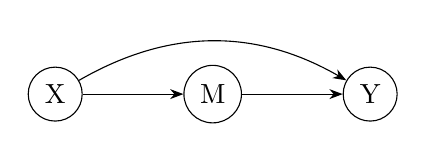
\begin{tikzpicture}[>=Stealth, node distance=2cm, on grid, auto]

        % Nodes
        \node (X) [draw, circle] {X};
        \node (M) [draw, circle, right=of X] {M};
        \node (Y) [draw, circle, right=of M] {Y};
      
        % Arrows
        \draw[->] (X) -- (M);
        \draw[->] (M) -- (Y);
        \draw[->] (X) to[bend left] (Y);
      
      \end{tikzpicture}
      \caption{Causal diagram showing $M$ mediating the effect of $X$ on $Y$.}    
      \label{fig:simp_med}
\end{figure}

We define the counterfactual $Y_x$ as the value $Y$ would assume when $X=x$. Similarly, write $M_x$ for the value $M$ would assume when $X=x$. Next, write $Y_{x,m}$ for the value $Y$ would assume if $X$ and $M$ were set to $x$ and $m$ respectively. Combining these ideas, we get the ``nested counterfactual'' $Y_{x, M_{x'}}$, which is the value of $Y$ when $X=x$ and $M$ is set to whatever it would have been when $X=x'$. It is common to link ordinary and nested conterfactuals by making the consistency assumption, which states $Y_x = Y_{x, M_x}$. Note that if $x \neq x'$ then the nested counterfactual is necessarily unobservable. It is nevertheless possible, given certain assumptions, to estimate the expected values of ordinary and nested counterfactuals. Section \ref{sec:ID} goes into detail on the identification of expected counterfactuals with estimable quantities.

There are three main types of mediation effect: total, direct and indirect, although the scale on which these are measured can vary. For concreteness, we focus here only on effects defined as differences; i.e., those of the form $Y_{x_1, M_{x_1'}} - Y_{x_2, M_{x_2'}}$. Extending our results to effects defined on different scales (e.g. ratios) is straightforward; see Section \ref{sec:med_effs}.

Proceeding now to the definitions, we set the total effect of $X$ on $Y$ to be $TE(x, x') = EY_x - EY_{x'}$. The direct effect is $DE(x, x') = Y_{x, M_{x'}} - Y_{x', M_{x'}}$, and the indirect effect is $IE(x, x') = Y_{x, M_{x}} - Y_{x, M_{x'}}$. See, e.g., \citet{Pea12} for motivation and discussion of these definitions.





\subsection{Identification and Modelling of Expected Counterfactuals}
\label{sec:ID}

A fundamental problem of causal inference is that we can only ever observe one counterfactual outcome on a particular individual. In mediation analysis, this problem is even worse, since many of our definitions involve the nested counterfactual, $Y_{x, M_{x'}}$, which when $x \neq x'$ cannot be observed on any individual. Nevertheless, \citet{Ima10I} give conditions under which the population average of a nested counterfactual can be expressed in terms of conditional expectations, possibly conditional on one or more additional covariates, $W$. Specifically, their Theorem 1 states that, under a condition they call ``Sequential Ignorability'', we can write
%
\begin{equation}
    \bE (Y_{x, M_{x'}} | W=w) = \bE_M \left[ \bE_Y \left( Y | X=x, M, W=w \right) | X=x', W=w \right]. \label{eq:ID}
\end{equation}
%
In fact, their Theorem 1 is somewhat more general, giving an expression for the density of the nested counterfactual rather than its expected value. We henceforth assume that Sequential Ignorability is satisfied by the variables in our model.

Using Equation (\ref{eq:ID}), we can estimate expected nested counterfactuals by working with the more tractable conditional expectations of $Y$ and $M$. We model the latter using regression, either linear or logistic depending on the forms of $Y$ and $M$. For concreteness, we take $Y$ and $M$ to both be binary. The extension of our method to continuous outcome and/or mediator is straightforward \textcolor{red}{(comment on sums $\rightarrow$ integrals and quadrature?)}. In this case, Equation (\ref{eq:ID}) has a particularly simple form:
%
\begin{multline}
    \bE (Y_{x, M_{x'}} | W=w) = \bP \left( Y=1 | X=x, M=1, W=w \right) \bP(M=1 | X = x', W=w) \\ + \bP \left( Y=1 | X=x, M=0, W=w \right) \bP(M=0 | X = x', W=w). \label{eq:ID_bin}
\end{multline}
%
We estimate the conditional probabilities on the right-hand side of Equation (\ref{eq:ID_bin}) using logistic regression. Note that we must fit two models: one to predict $M$ using $X$ and $W$, and another to predict $Y$ using $M$, $X$ and $W$.

We extend this regression modelling with the introduction of random effects \citep[see, e.g.][]{Dem04}. Specifically, we include random effects for the intercept and $X$ in our model for $M$, and for the intercept, $X$ and $M$ in our model for $Y$. Let $U$ and $V$ be the random effects for our models of $Y$ and $M$ respectively. We can re-write Equation (\ref{eq:ID_bin}) as
%
\begin{align}
    \bE (Y_{x, M_{x'}} | W=w) = & \left[\bE_U \bP \left( Y=1 |U, X=x, M=1, W=w \right) \right. \cdot \label{eq:ID_bin_ran}\\
    &  \left. \bE_V \bP(M=1 |V, X = x', W=w)\right] + \nonumber \\ 
    & \left[ \bE_U \bP \left( Y=1 |U, X=x, M=0, W=w \right) \right. \cdot \nonumber \\
    & \left. \bE_V \bP(M=0 |V, X = x', W=w) \right]. \nonumber 
\end{align}
%
We model the random effects $U$ and $V$ as normally distributed, allowing for correlation between effects from the same model, but assuming independence between models (i.e. $U \indep V$). Let $U \sim N(0, \Gamma_Y)$ and $V \sim N(0, \Gamma_M)$.


\subsubsection{Expanding One Term in Equation (\ref{eq:ID_bin_ran})}

We derive an expression for the first term in Equation \eqref{eq:ID_bin_ran}, then report results for the other three terms \textcolor{red}{(awk)}. 

First, write $\eta_Y = (\alpha_0 + \alpha_X x + \alpha_M m + A_W^T w) + (U_0 + U_X x + U_M m)$ for the linear predictor of $Y$ based on $X$, $M$ and $W$. Let $\mu_Y = \alpha_0 + \alpha_X x + A_W^T w$, so that the fixed-effects component of $\eta_Y$ is $\mu_Y + \alpha_M m$, and let $\xi_Y = U_0 + U_X x + U_M m$ be the random-effects component of $\eta_Y$. For convenience, we will also write $\gamma^2_Y(c_1, c_2, c_3) = (c_1, c_2, c_3) \Gamma_Y (c_1, c_2, c_3)^T$, so that $\bV \xi_Y = \gamma^2_Y(1, x, m)$ (recall that $\Gamma_Y$ is the covariance matrix of $U$).

It is a well-known fact about logistic regression that
%
\begin{equation}
    \bP \left( Y=1 |U, X=x, M=1, W=w \right) = \left[1 + \exp(-\eta_Y)\right]^{-1},
\end{equation}
%
so the first term in Equation (\ref{eq:ID_bin_ran}) can be written as
%
\begin{align}
    \bE_U \bP \left( Y=1 |U, X=x, M=1, W=w \right) & = \int \frac{\phi_3(u; 0, \Gamma_Y)}{1 + \exp(-\eta_Y)} du, \label{eq:pY1_bad}
\end{align}
%
where $\phi_d$ is the $d$-variate normal density. A straightforward change of variables gives us the alternative expression
%
\begin{align}
    \bE_U \bP \left( Y=1 |U, X=x, M=1, W=w \right) & = \int \frac{\phi_1(z; 0, 1)}{1 + \exp(-\mu_Y - \alpha_M - \gamma_Y(1, x, 1) z)} dz. \label{eq:pY1}
\end{align}
%
Importantly, the integral in Equation (\ref{eq:pY1}) is univariate (and thus amenable to numerical evaluation using quadrature). This integral arises often enough that we give it a name. Let
%
\begin{equation}
    \Psi(a, b) = \int \frac{\phi(z; 0, 1)}{1 + \exp(-a - b z)} dz.
\end{equation}
%
We can now write the first term in \eqref{eq:ID_bin_ran} compactly as
%
\begin{equation}
    \bE_U \bP \left( Y=1 |U, X=x, M=1, W=w \right) = \Psi(\mu_Y + \alpha_M, \gamma_Y(1, x, 1))
\end{equation}
%
Returning now to the other terms in Equation \eqref{eq:ID_bin_ran}, similar expressions hold. Write $\eta_M = (\beta_0 + \beta_X x + B_W^T w) + (V_0 + V_X x)$ for the linear predictor of $M$ based on $X$ and $W$. Write $\mu_M = \beta_0 + \beta_X x + B_W^T w$ and $\xi_M = V_0 + V_X x$ for the fixed and random components respectively of $\eta_M$. Finally, write $\gamma^2_M(c_1, c_2) = (c_1, c_2) \Gamma_M (c_1, c_2)^T$, so that $\bV \xi_M = \gamma^2_M(1, x)$ ($\Gamma_M$ is the covariance matrix of $V$). We can now write the expected counterfactual in \eqref{eq:ID_bin_ran} as
%
\begin{align}
    \bE (Y_{x, M_{x'}} | W=w) = & \left[  \Psi(\mu_Y + \alpha_M, \gamma_Y(1, x, 1)) \cdot \Psi(\mu_M , \gamma_Y(1, x')) \right] + \label{eq:Psi_bin_ran}\\
    & \left[ \Psi(\mu_Y, \gamma_Y(1, x, 0)) \cdot \Psi(- \mu_M , \gamma_Y(1, x')) \right] \nonumber
\end{align}
%
Recall that each term in \eqref{eq:Psi_bin_ran} is a univariate integral, and can thus be accurately evaluated using standard numerical quadrature routines available in most software packages.

\subsection{Estimation and UQ}
\label{sec:CF_UQ}

Although not obvious from our notation, Equation \eqref{eq:Psi_bin_ran} depends only on the parameters of our two regression models (as well as the levels of our covariates, $x$, $x'$ and $w$). Estimation of the expected counterfactual thus proceeds by first fitting these two regression models to our data, then plugging-in our estimates of the two sets of model parameters to Equation \eqref{eq:Psi_bin_ran}. More precisely, if we re-write \eqref{eq:Psi_bin_ran} as
%
\begin{equation}
    \bE (Y_{x, M_{x'}} | W=w) = \kappa(x, x', w; \alpha, \Gamma_Y, \beta, \Gamma_Y) \label{eq:kappa},
\end{equation}
%
then our estimate of this expected counterfactual is
\begin{align}
    \hat{\bE} (Y_{x, M_{x'}} | W=w) &= \kappa(x, x', w; \hat{\alpha}, \hat{\Gamma}_Y, \hat{\beta}, \hat{\Gamma}_M) \label{eq:kappa_hat}\\
    &=: \hat{\kappa}(x, x', w)
\end{align}
%
We often omit the parameters from $\kappa$, and $w$ from both $\kappa$ and $\hat{\kappa}$. 

Uncertainty quantification for our estimator, $\hat{\kappa}$, proceeds by the $\delta$-method \citep[see, e.g.,][]{vdV98}. We first get asymptotic covariance matrices for estimators of our two sets of regression parameters. Next, we stack these two covariances into a single $2\times 2$ block-diagonal matrix (\hl{assuming asymptotic independence between models, see} \citealp{Bau06}), then pre- and post-multiply by the Jacobian of $\kappa$. From traditional M-estimator theory, the asymptotic covariance of our regression estimators is approximately the inverse Hessian of their respective objective functions at the maximizers. These objective functions differ from log-likelihoods only in that Laplace's method is used to approximate the marginal likelihood of the data from its joint likelihood with the random effects.

We omit here an explicit formula for the asymptotic covariance of $\hat{\kappa}$, \textcolor{red}{but one can be found in our \texttt{R} package\footnote{Name idea: \texttt{MultMedUQ}?}. See also the supplemental material for an accompanying derivation.} For concreteness however, write $\sqrt{n} (\hat{\kappa}(x, x') - \kappa(x, x')) \rightsquigarrow N(0, \lambda^2(x, x'))$. We will often also need the limiting covariance of $\kappa$ evaluated at two sets of values for $x$ and $x'$. In this case we write $\rho(x_1, x'_1; x_2, x'_2)$ for the asymptotic correlation between $\hat{\kappa}(x_1, x'_1)$ and $\hat{\kappa}(x_2, x'_2)$.


\subsection{Mediation Effects}
\label{sec:med_effs}

Recall that we define the three mediation effects, total, direct and indirect, in terms of expected counterfactuals of the form given in Equation \eqref{eq:kappa}. Estimation and uncertainty quantification for mediation effects thus follows immediately from the corresponding analysis of expected counterfactuals. Recall from Section \ref{sec:MA_defns} that, if we define effects as differences, then formulas for the three mediation effects are given in Table ???? (\textcolor{red}{Add a table at end of Section \ref{sec:MA_defns}}). Since these mediation effects are all linear combinations of the expected counterfactuals, their asymptotic variances are easily obtained. See Table \ref{tab:med_diffs}. Alternatively, these asymptotic variances can be derived by applying the $\delta$-method to the map from various $\hat{\kappa}$s to the mediation effect. For example, the total effect can be obtained by first computing the asymptotic covariance matrix of $\hat{\kappa}(x,x)$ and $\hat{\kappa}(x',x')$, then pre- and post-multiplying by the gradient of the map $(\kappa_1, \kappa_2) \mapsto \kappa_1 - \kappa_2$.

\begin{table}
    \centering
    \begin{tabular}{|c|c|c|}
        \hline
        Effect & Definition & Asymptotic Variance\\
        \hline
        Total & $\kappa(x, x) - \kappa(x', x')$ &  $\lambda^2(x, x) + \lambda^2(x', x') - 2 \lambda(x, x)  \lambda(x', x')  \rho(x, x; x', x')$\\
        Direct & $\kappa(x, x') - \kappa(x', x')$ & $\lambda^2(x, x') + \lambda^2(x', x') - 2 \lambda(x, x')  \lambda(x', x')  \rho(x, x'; x', x')$\\
        Indirect & $\kappa(x, x) - \kappa(x, x')$ & $\lambda^2(x, x) + \lambda^2(x, x') - 2 \lambda(x, x)  \lambda(x, x')  \rho(x, x; x, x')$\\
        \hline
    \end{tabular}
    \caption{Mediation effects defined on difference scale.}
    \label{tab:med_diffs}
\end{table}

Suppose instead that mediation effects are desired on a different scale, such as risk-ratios or odds-ratios for binary outcomes. In this case, we adjust the definitions of the various effects accordingly, and estimate each expected counterfactual $\kappa$ with the corresponding plug-in estimator, $\hat{\kappa}$. Uncertainty quantification proceeds by applying the $\delta$-method to the function which maps various $\hat{\kappa}$s to the desired mediation effect. For example, the limiting variance of the total effect on risk-ratio scale can be obtained by first computing the asymptotic covariance matrix of $\hat{\kappa}(x,x)$ and $\hat{\kappa}(x',x')$, then pre- and post-multiplying by the gradient of the map $(\kappa_1, \kappa_2) \mapsto \kappa_1 / \kappa_2$. Formulas for these asymptotic variances tend to be quite long, but are easily implemented computationally (see our package ????).

While the above discussion focuses on estimation of each mediation effect individually, it is straightforward to extend our analysis to simultaneous estimation of, for example, the total, direct and indirect effects on a single scale. This has the advantage of estimating covariances between mediation effects, rather than just the effects' marginal variances.



\section{Empirical Investigation}

\begin{outline}
    \1 Monte Carlo study
        \2 Proof of concept
        \2 Explore robustness. See \citet{Sam23} for inspiration.
    \1 Real data
        \2 Trust study dataset? (this will be the focus of an applied paper)
\end{outline}

\bibliography{../Bib-Exact_Asymptotics}

\end{document}